\chapter{Design and implementation}
In this chapter the design and system architecture of the product will be presented. The reader will learn how the different components of the product are put together, and how the design of the application was planned.

\section{System architecture}
	The design was divided into several modules:
	\begin{itemize}
		\item{Bluetooth connection between the Android and the Arduino}
		\item{Synchronization with the local SQLite database}
		\item{Android application view (General user interface)}
		\item{A service that contains the protocol for installing over-the-air}
	\end{itemize}
	\vspace{0.2in}
	
	The system design was implemented such that further development should be as modular and easy as possible. Therefore it was designed as a plugin-like system where you easily can implement your own protocols against a desired device, e.g. Raspberry Pi. Currently the application only supports the STK500v1 protocol and therefore only connections with Arduino devices. With some work, compatibility with other STK500-based devices can implemented. be The design for the connection to other devices was done as shown in Figure~\ref{fig:btconnection_service_stk500}.\\

	\begin{figure}[H]
	\centering
	\hspace*{-0.75in}
	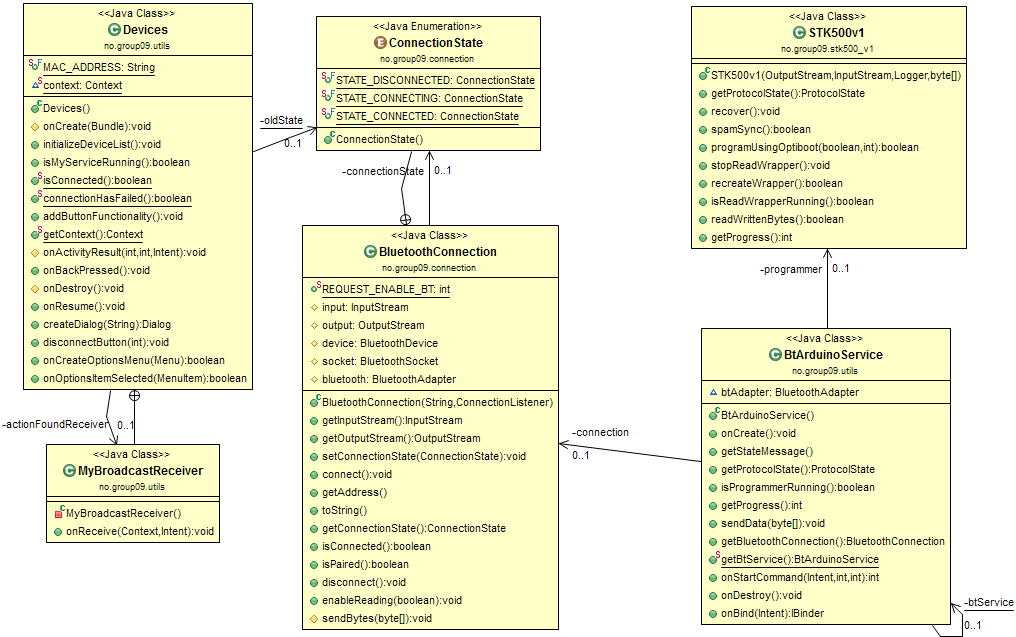
\includegraphics[scale=0.85]{images/UML/btconnection_service_stk500.png}
	\caption[BT connection in service]{The Bluetooth connection is stored and managed in a service that provides the STK500 protocol.}
	\label{fig:btconnection_service_stk500}
	\end{figure}

	\textit{Devices}, as shown in Figure~\ref{fig:btconnection_service_stk500}, is an activity that manages the discovered Bluetooth devices. A device is discovered by listening to the Bluetooth API on the Android. This happens in the \textit{MyBroadcastReceiver} which works like a listener. When this listener gets notified with a device as input, the discovered device will be put in a list in \textit{Devices}.\\

	If the user choose to connect to a device from the list of discovered devices, a service (\textit{BtArduinoService}) will be created. This service will create the \textit{BluetoothConnection} that manages the connection between the Android device and a Bluetooth device. The service uses \textit{STK500v1} for transferring data over the \textit{BluetoothConnection} to the connected device.\\

	To add support for other microcontrollers than Arduino, only few changes to \textit{Devices} would have to be made.Another service and a protocol communicating with a desired device must be implemented. If the added protocol(s) should coexist with STK500v1, support for multiple simultaneous services must also be implemented as well. Since this project only considered connections between Android and Arduino, only the STK500v1 protocol and one service was implemented.\\

	The overall design solution for multiple connections is described in Figure~\ref{fig:otaarchitecture}.\\
	\begin{figure}[H]
	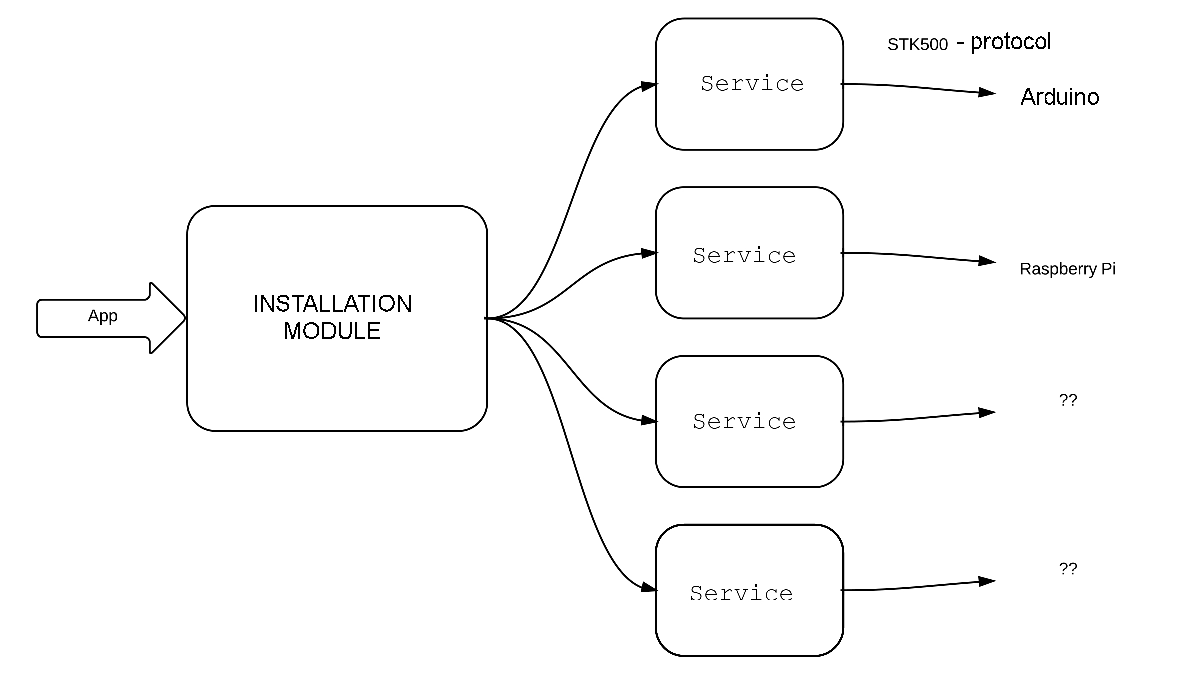
\includegraphics[scale=0.7]{figures/OTAArchitecture.pdf}
	\caption[Over The Air Architecture]{The installation module is a class that manages all the services that the application may support. Each service has a protocol for installing software over-the-air to a desired microcontroller.}
	\label{fig:otaarchitecture}
	\end{figure}

	The overall system architecture as shown in Figure~\ref{fig:systemarchitecture} and Figure~\ref{fig:adddevicescreenuml} illustrates the core components of the system and the relationship between these components. The \textit{Market Application} is the centre of the application and is where most of the GUI and functionality visible to the user is shown. \textit{Device List} is the list of devices that the user can choose from and connect to. This is also the location of the \textit{Add Device} functionality, where the user can connect to a device in an alternative way (QR Code or MAC-address).\\

	\begin{figure}[H]
	\centering
	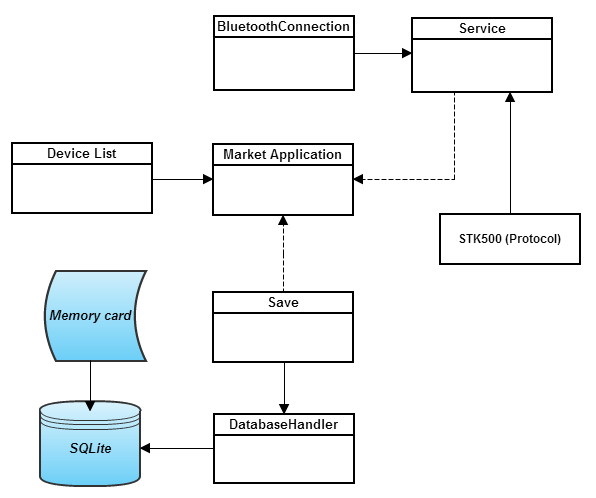
\includegraphics[scale=0.8]{images/System_architecture.png}
	\caption[System Architecture]{This shows the overall system architecture with the most important components.}
	\label{fig:systemarchitecture}
	\end{figure}

	\begin{figure}[H]
	\centering
	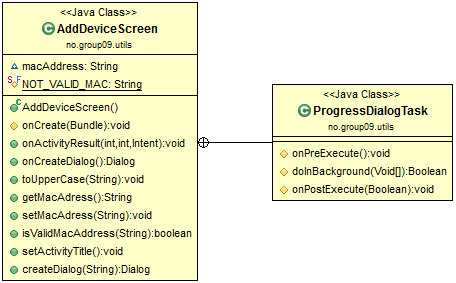
\includegraphics[scale=0.85]{images/UML/adddevicescreen.png}
	\caption[UML - AddDeviceScreen]{This is a UML diagram of the \textit{Add Device Screen}. When QR-reader or input serial is chosen, a new asynchronous task is started that handles the Bluetooth connection process.}
	\label{fig:adddevicescreenuml}
	\end{figure}

	The \textit{Service} holds and manages the Bluetooth connection (\textit{BluetoothConnection}) and is communicating with the protocol for installing apps on the microcontroller. \\

	The \textit{Memory card} represents the local storage solution on the mobile phone where the database is stored. SQLite was used as the database engine because it is common and easy to implement on Android.\\

	\textit{DatabaseHandler} is a class for taking care of the SQL transactions and is the access point for communication with the database. A helper class called \textit{Save} is used for easy access to the \textit{DatabaseHandler}.
	When the application communicates with the \textit{Save} module, the database communicates with the DatabaseHandler. The \textit{Save} class can be created from any class in the application. It ensures that only a single instance of the \textit{DatabaseHandler} can be instantiated and handles insertions and queries.

	\textit{Save} was created because it can be initialized and created everywhere in the application (in optional Java classes) and makes sure it is only one instance of the \textit{DatabaseHandler}.

	\subsection{Browse shop}
	This is the shop where the user can see the $\mu$C apps, choose categories and swipe through different fragments. In  Figure~\ref{fig:categoriesuml} one can see the \textit{MainActivity} which is the activity for the category selection of the shop. When a category is selected, a new activity \textit{MainFragmentActivity} (see Figure~\ref{fig:maingui}) is started with the Intent about which category was selected.

	\begin{figure}[H]
	\centering
	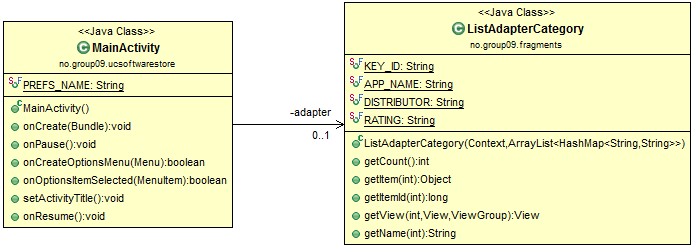
\includegraphics[scale=0.85]{images/UML/categories.png}
	\caption[UML - Categories]{The \textit{MainActivity} is an activity with a \textit{ListView} that uses \textit{ListAdapterCategory} as an adapter. When a category is selected, the \textit{MainFragmentActivity} is started with Intent about which category was selected.}
	\label{fig:categoriesuml}
	\end{figure}

	In Figure~\ref{fig:maingui} the \textit{MainFragmentActivity} is started when a category is selected. This activity creates a \textit{FragmentPagerAdapter} that manages the fragments. One fragment is one of the views that can be swiped through. \textit{All} and \textit{TopHits} are these fragments. Each fragment consist of a list, and have an \textit{Adapter} for this list (\textit{ListAdapter}).

	\begin{figure}[H]
	\hspace*{-1.0in}
	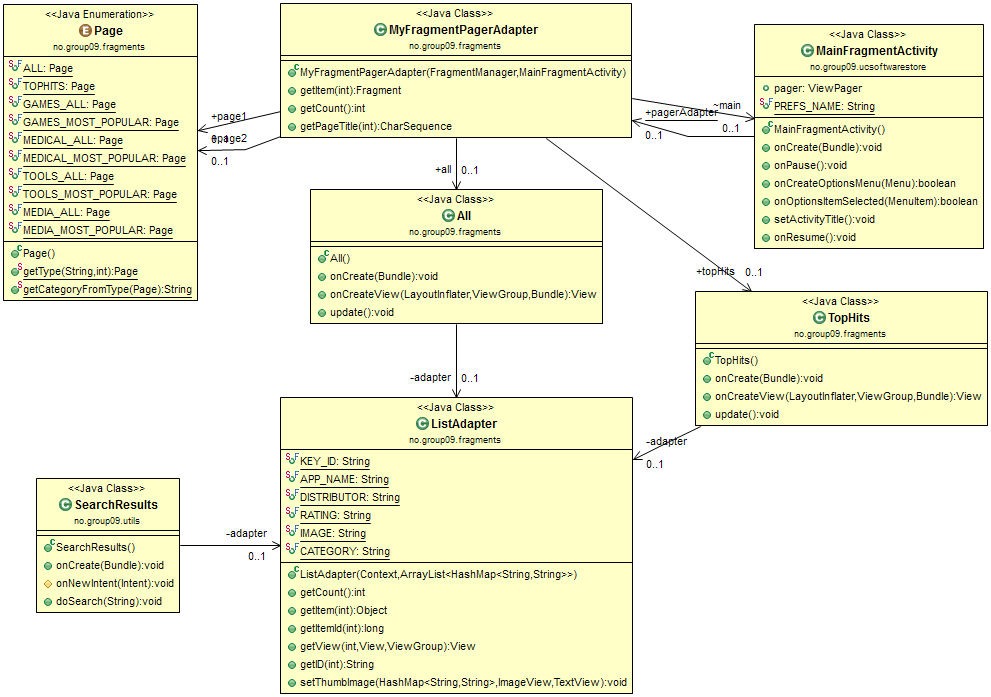
\includegraphics[scale=0.55]{images/UML/main.png}
	\caption[UML - Main GUI]{Here one can see a \textit{FragmentPagerAdapter} that manages all the fragments. Each fragment uses a \textit{ListAdapter} that structures the list items.}
	\label{fig:maingui}
	\end{figure}

	The \textit{Page} enum is used to tell \textit{MyFragmentPagerAdapter} which category that should be shown in \textit{All} and \textit{TopHits} fragments. This enum is sent as an intent to the \textit{MainFragmentActivity} when started. When a category is chosen, the content in \textit{All} and \textit{TopHits} are filtered by only showing applications that belongs to the selected category.\\

	\textit{SearchResults} is a class that contains a list of search results ($\mu$C applications) from a search. This class is an activity that has a list like the other fragments, and therefore uses the same list adapter as \textit{All} and \textit{TopHits}. 

	When a specific $\mu$C app is chosen, a new activity is started: \textit{AppView}. This class contains the information about the chosen app and presents it to the user. From this screen the user can choose to install the app on the connected Arduino.

	\subsection{STK500v1}
	In Figure~\ref{fig:stk500v1uml} the general design of the protocol component is shown. The \textit{STK500v1} class
    handles most of the logic and actual programming; this is the class called upon by the application when
    an app is to be uploaded. The \textit{Constants} class holds important commands and responses used when communicating
    with the Arduino. The \textit{Hex} class deals with interpreting and verifying the app to be programmed. It provides the raw bytes requested by the protocol class.\\

    The rest are for abstracting and dealing with reading from the Bluetooth connection; the current
    implementation allows for avoiding blocking by only reading buffered bytes. The Reader behaves differently while reading or during timeouts, based on a state pattern implementation. As shown, the different states are both
    states and readers.\\

	\begin{figure}[H]
	\hspace*{-1.0in}
	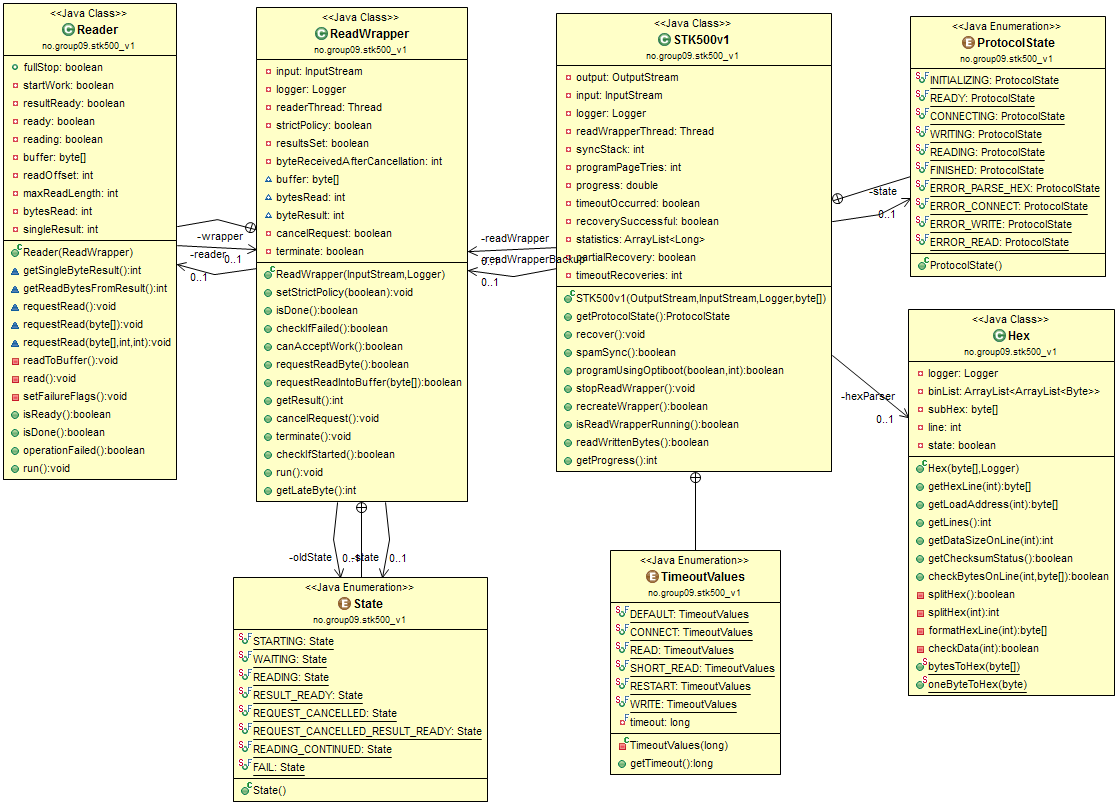
\includegraphics[scale=0.58]{images/UML/stk500v1.png}
	\caption[UML - Protocol]{The most important classes used for programming}
	\label{fig:stk500v1uml}
	\end{figure}

	In Figure~\ref{fig:stk500_sequence_diagram} a simplified view of the programming process is shown. Here the \textit{ArduinoStore} is a representation of any application requesting an app to be uploaded to the Arduino. The \textit{Arduino} represents a microcontroller to be programmed.\\
	
	Note that the \textit{IReader} has already been instantiated before the starting call, and that stopping doesn't
	destroy the object.\\
	
	Most of the simplification occurs within the programming loop, as several different types of commands
	are sent to the device, depending on the responses received; for details on this communication, see the AVR061 documentation~\cite{AVR061}. Communication details with the \textit{Hex} class and \textit{IReader}-related classes have also been reduced slightly in the diagram.\\
	
	\begin{figure}[H]
	\hspace*{-1.0in}
	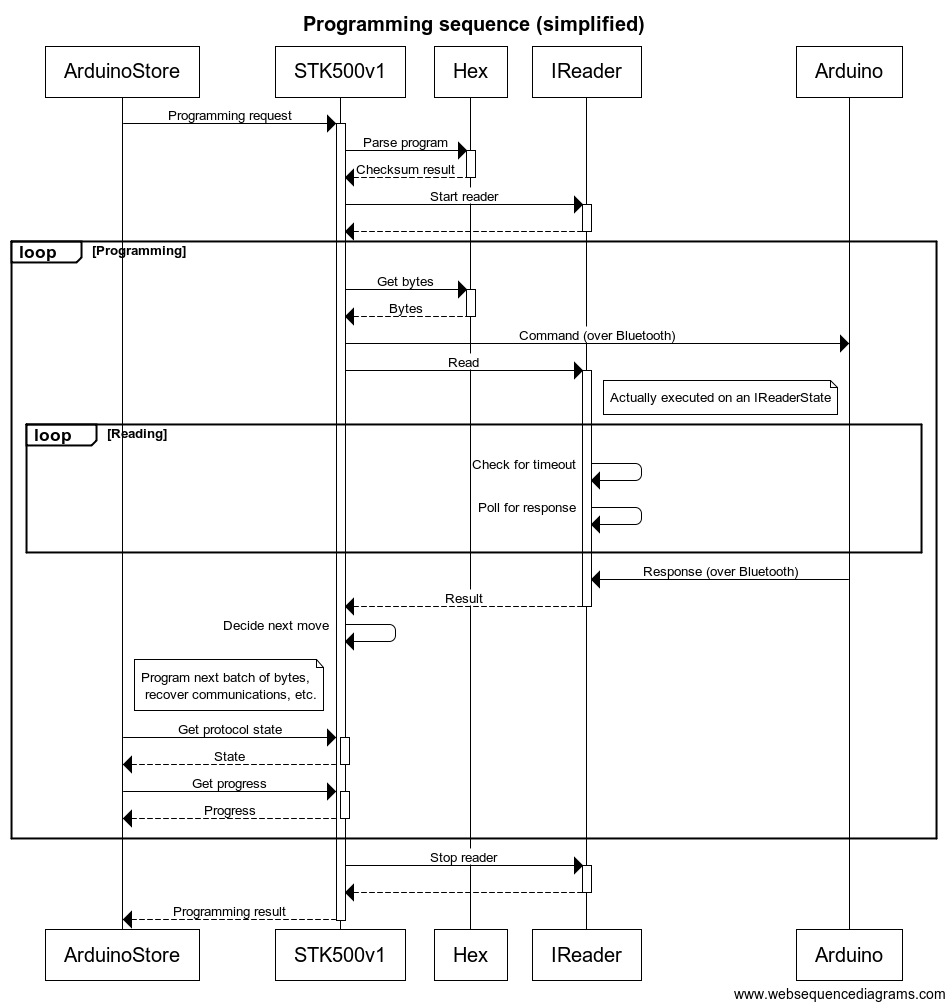
\includegraphics[scale=0.6]{images/Sequence_diagram.png}
	\caption[Sequence diagram for programming]{Sequence diagram of the programming process. The three classes in the middle are in the protocol library, \textit{ArduinoStore} represents an outside caller, and the \textit{Arduino} is a programmable microcontroller.}
	\label{fig:stk500_sequence_diagram}
	\end{figure}


\section{Design of the Android application}
One of the purposes of the Android application was to ease the process of installing PUIs on an Arduino for non-technical users. As described in section \ref{non-functional}, one of the requirements for the project was that people of all ages were supposed to understand how to use the application. This requirement put pressure on the design, as one has to make sure everyone were able to understand the different functions of the application.

\subsection{Design guide}
Before the programming of the Android application was started, a complete design guide was created. In this section the complete design of the application is presented. This guide was made primarily for two reasons:\\
\begin{itemize}
	\item{Presentation for the customer:} With a complete design guide it was possible to present the user interface of the application to the customer before it was programmed. This allowed for input from the customer at an early stage, when it was easier to change the design.
	\item{Avoid confusion:} A design guide reduces the amount of confusion and discussion regarding the appearance of the user interface. Because the design of the user interface was settled on before the programming had started, there was less need to discuss this along the way.
\end{itemize}
\vspace{6 mm}
During the project, some changes were made to the design. These changes can be viewed in Section \ref{designchanges}.

\paragraph{Screen 1a - Device list,} as shown in Figure \ref{fig:screen1a}, shows the list of available Arduino devices. In the final design the list of devices fills the whole screen, and the buttons and description text have switched places. When a device is pressed, a progress bar appears and stays on the screen until a valid Bluetooth connection with the chosen device is made.

\begin{figure}[H]
	\centering
		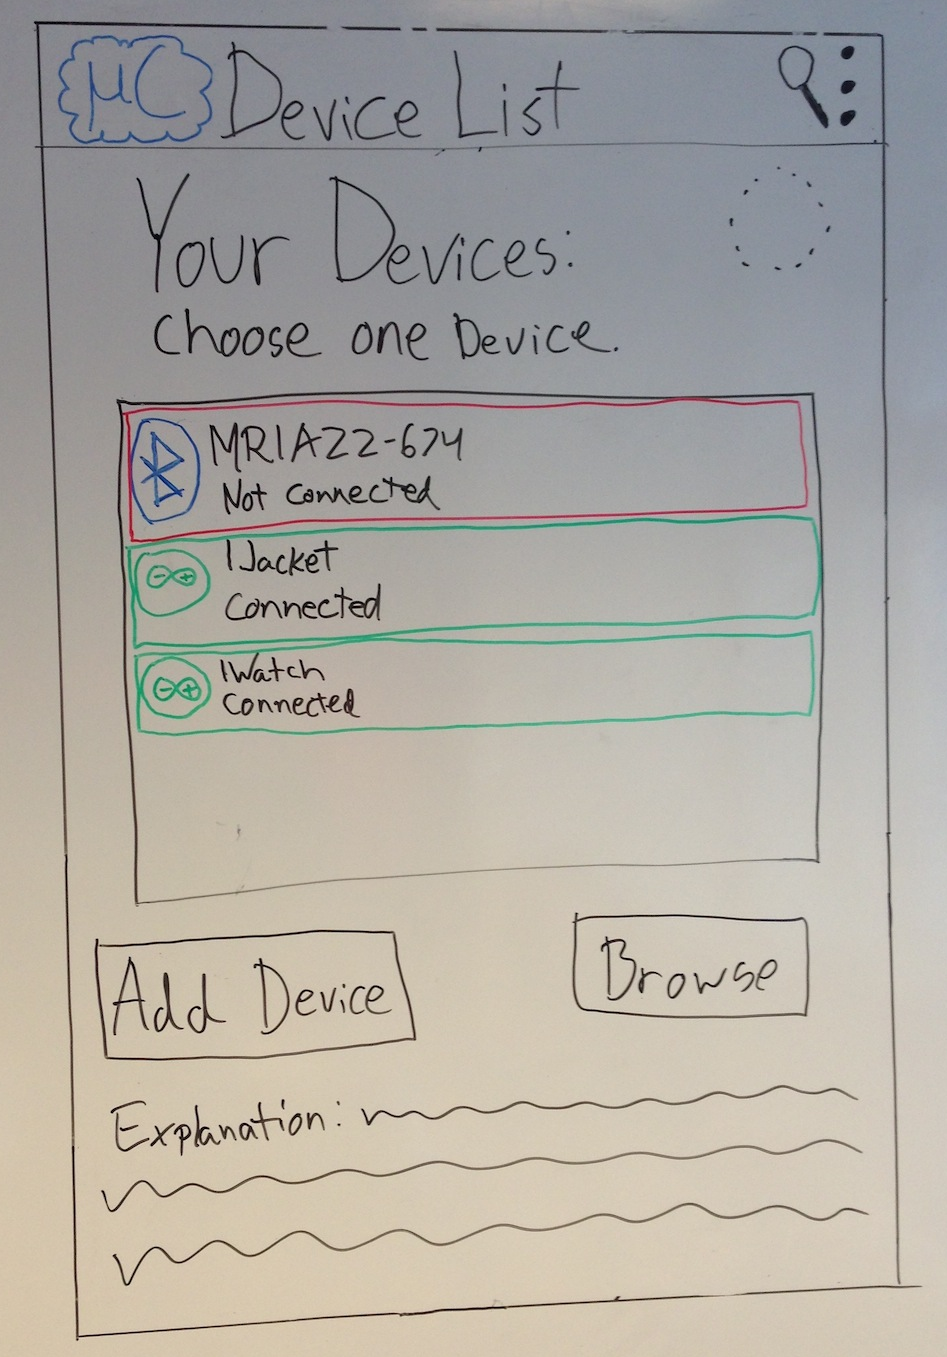
\includegraphics[scale=0.2]{images/Design_guide/Screen1a.png}
	\caption[Screen 1a - Device list]{The design for the device list of the discovered Bluetooth devices}
	\label{fig:screen1a}
\end{figure}


\paragraph{Screen 1b - Add device manually,} as shown in Figure \ref{fig:screen1b}, appears after pressing the ``Add device'' button in Screen 1a. It was chosen to remove the ``Bluetooth settings'' button, as it proved unnecessary. In the final design, this screen contains only the ``QR Code'' button and ``Input serial'' button, with a short description of the functionality of the button between them.

\begin{figure}[H]
	\centering
		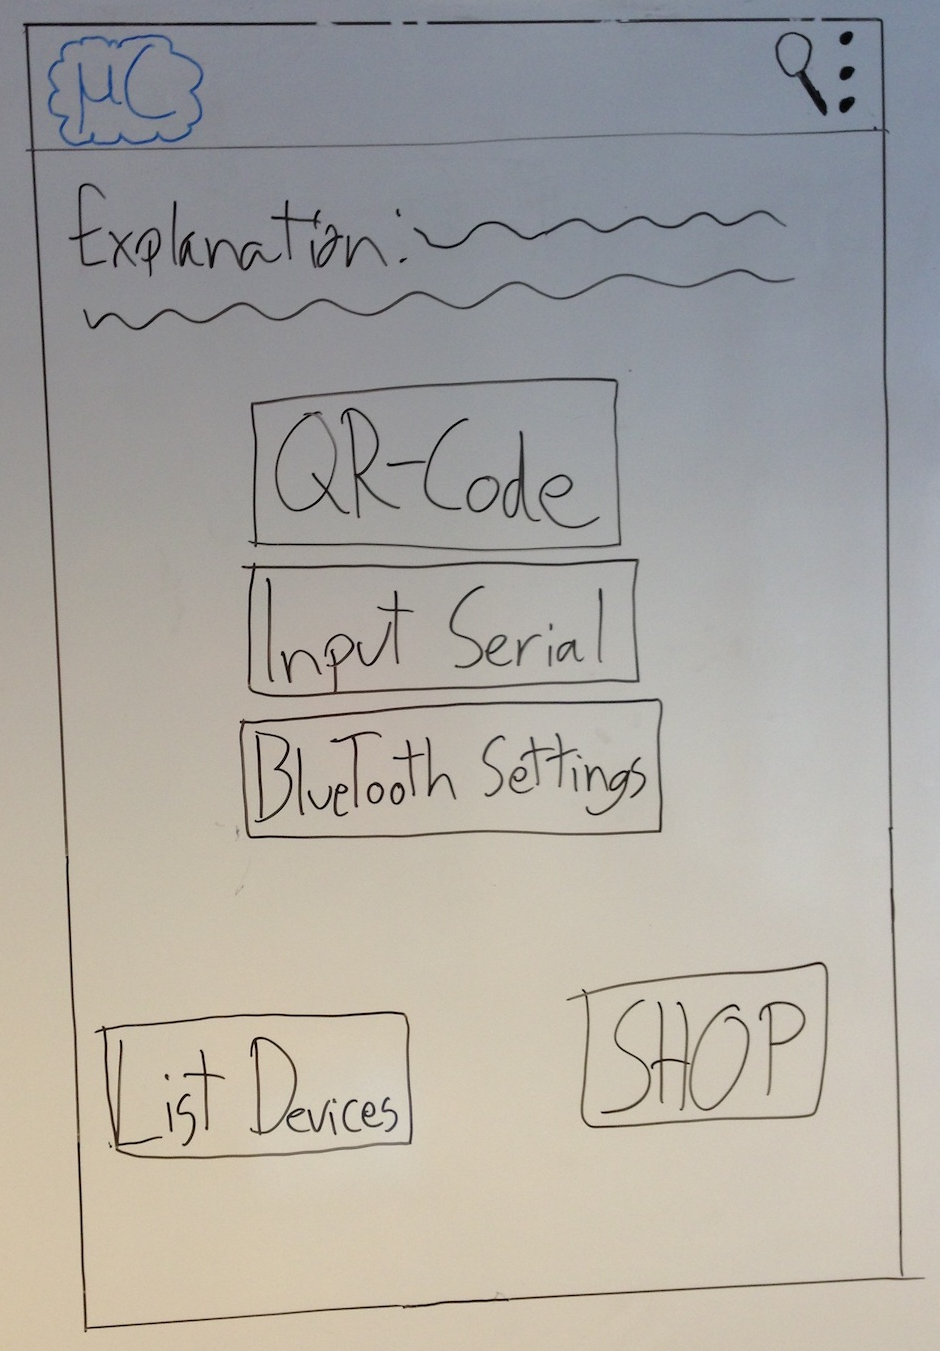
\includegraphics[scale=0.2]{images/Design_guide/Screen1b.png}
	\caption[Screen 1b - Add device manually]{The design for alternative methods to add devices}
	\label{fig:screen1b}
\end{figure}


\paragraph{Screen 1b-i - Input serial,} as shown in Figure \ref{fig:screen1bi}, appears when the ``Input serial'' button is clicked.

\begin{figure}[H]
\centering
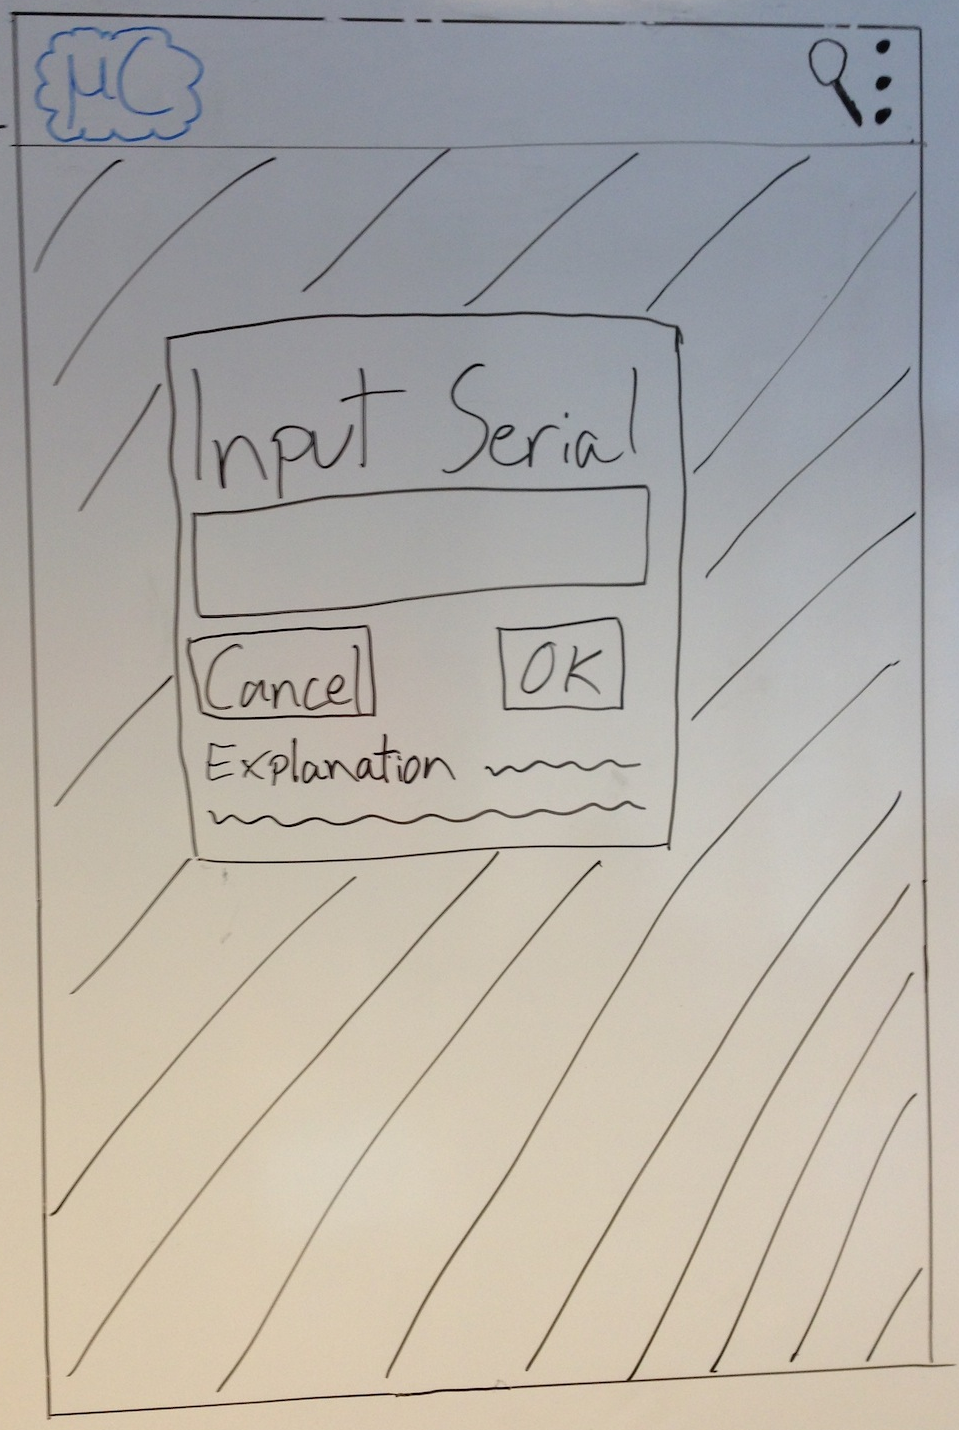
\includegraphics[scale=0.2]{images/Design_guide/Screen1b-i.png}
\caption[Screen 1b-i - Input serial]{The design for Input serial box.}
\label{fig:screen1bi}
\end{figure}


\paragraph{Screen 2a - Browse shop,} as shown in Figure \ref{fig:screen2a}, is a screen for browsing all the apps for Arduino in the shop. More categories have been added. The user can swipe to the left or right to sort the available applications in different ways. See next paragraph.

\begin{figure}[H]
\centering
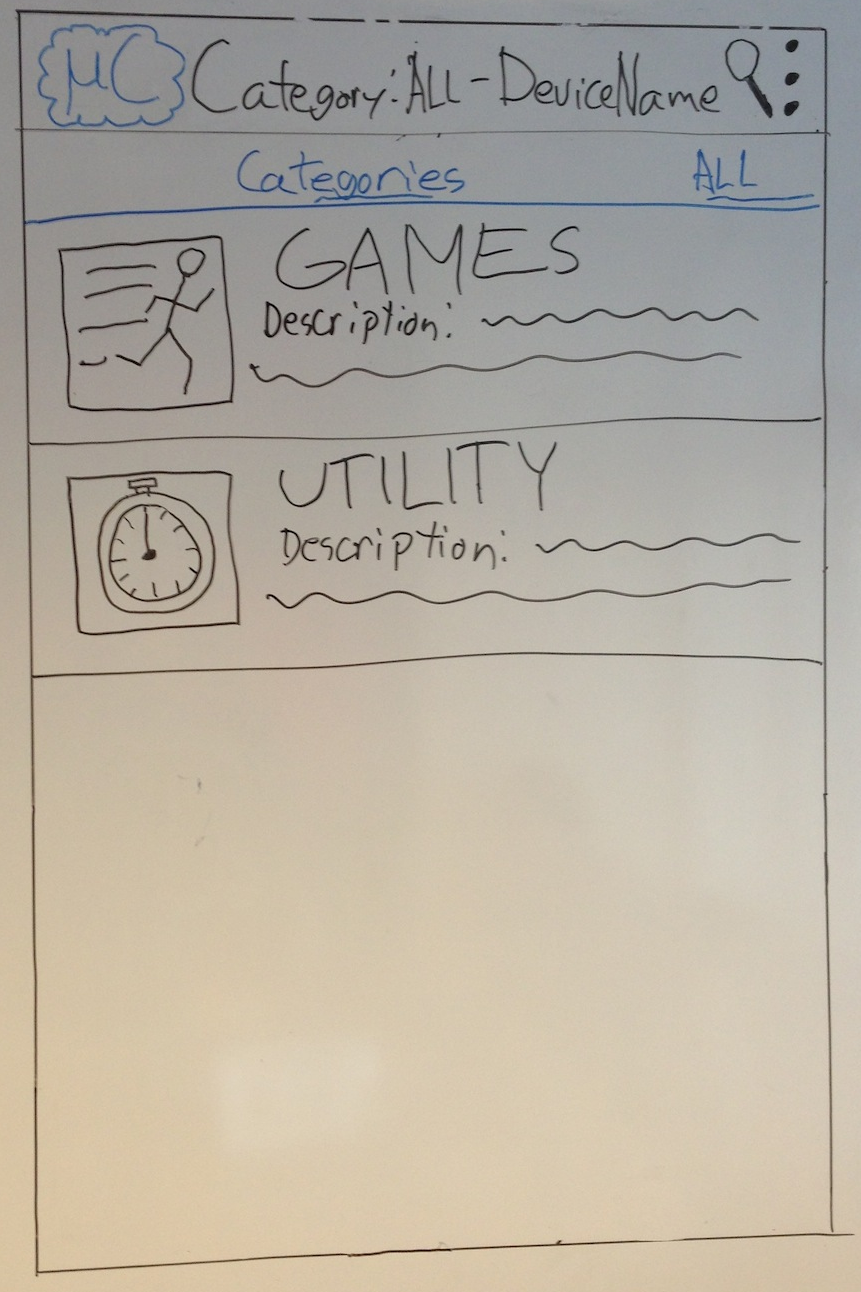
\includegraphics[scale=0.2]{images/Design_guide/Screen2a.png}
\caption[Screen 2a - Browse shop]{Design for category selection in the shop.}
\label{fig:screen2a}
\end{figure}


\paragraph{Screen 2b - Browse shop by category,} as shown in Figure \ref{fig:screen2b}, is a
 screen that shows a list of all applications in the chosen category. Category ``All'' is chosen.

\begin{figure}[H]
\centering
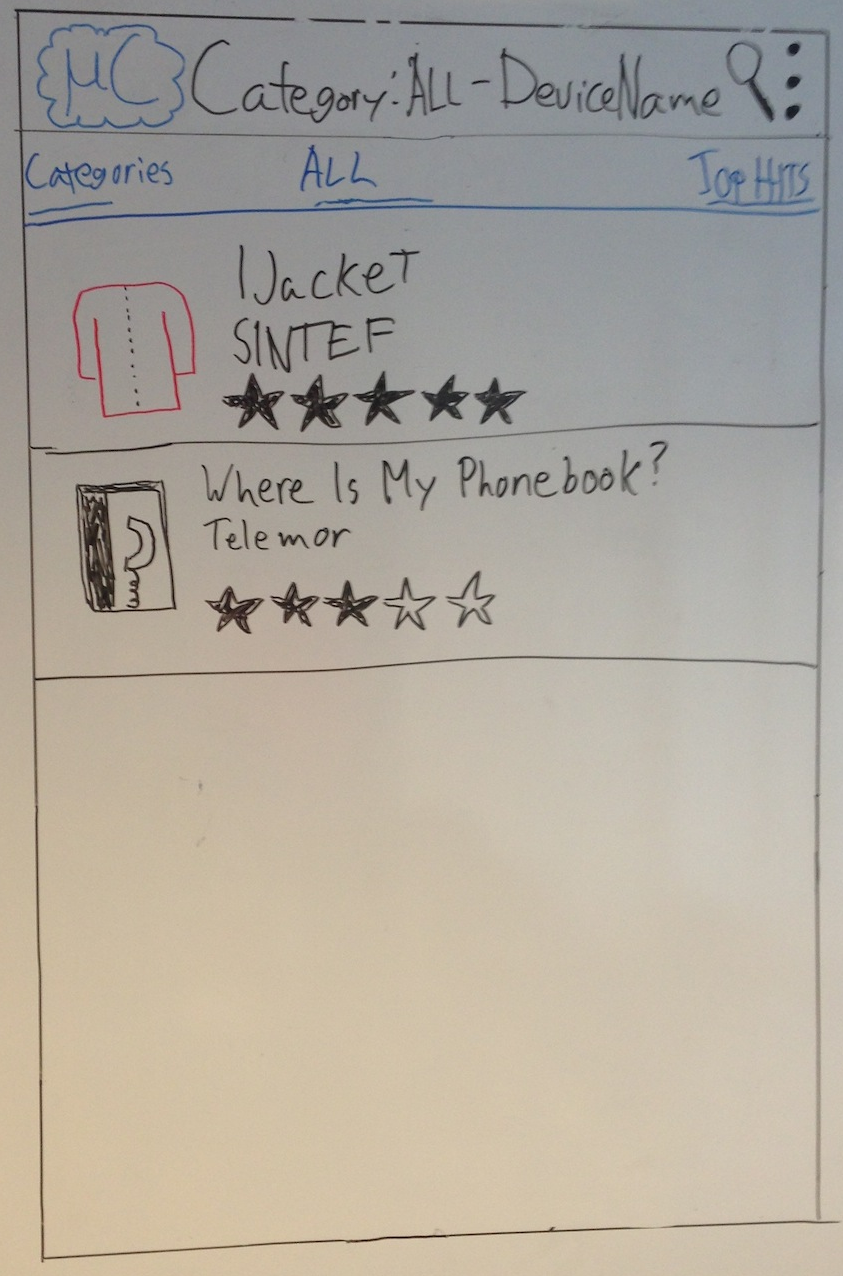
\includegraphics[scale=0.2]{images/Design_guide/Screen2b.png}
\caption[Screen 2b - Browse shop by category]{Design for the list of application that belongs to the selected category.}
\label{fig:screen2b}
\end{figure}


\paragraph{Screen 3a - Application view,} as shown in Figure \ref{fig:screen3a}, provides an overview of a chosen application. Small changes were needed, as the comments field and reviews were given a lower priority at mid-term.

\begin{figure}[H]
\centering
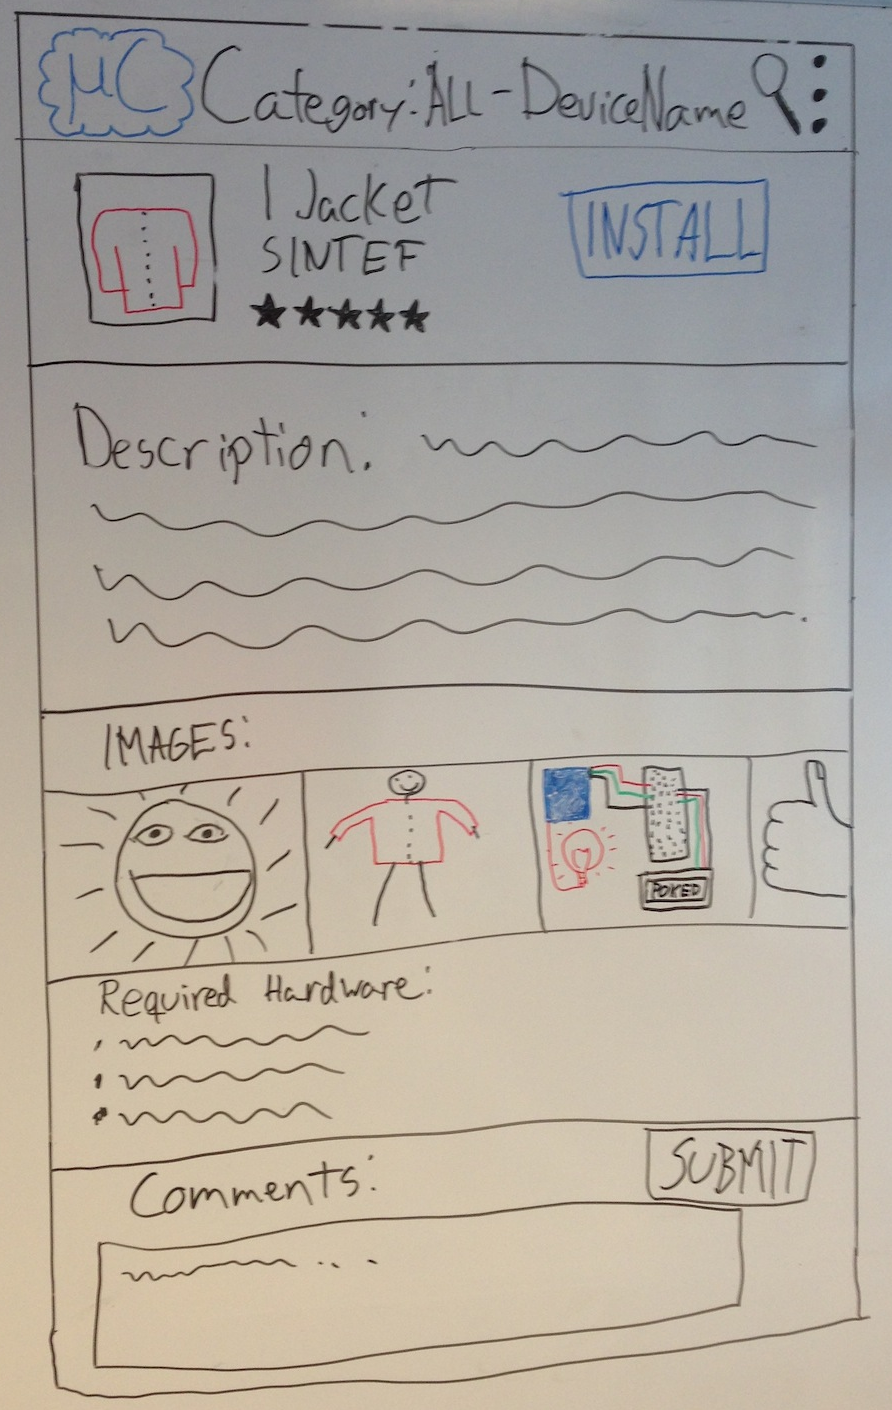
\includegraphics[scale=0.2]{images/Design_guide/Screen3a.png}
\caption[Screen 3a - Application view]{The design for application view. This is the screen you see when you look at the details about an application}
\label{fig:screen3a}
\end{figure}


\paragraph{Screen 3a-i - Installation confirmation,} as shown in Figure \ref{fig:screen3ai}, is a 
screen that appears when the ``Install'' button in Screen 3a is pressed. Shows the name of the chosen device.

\begin{figure}[H]
\centering
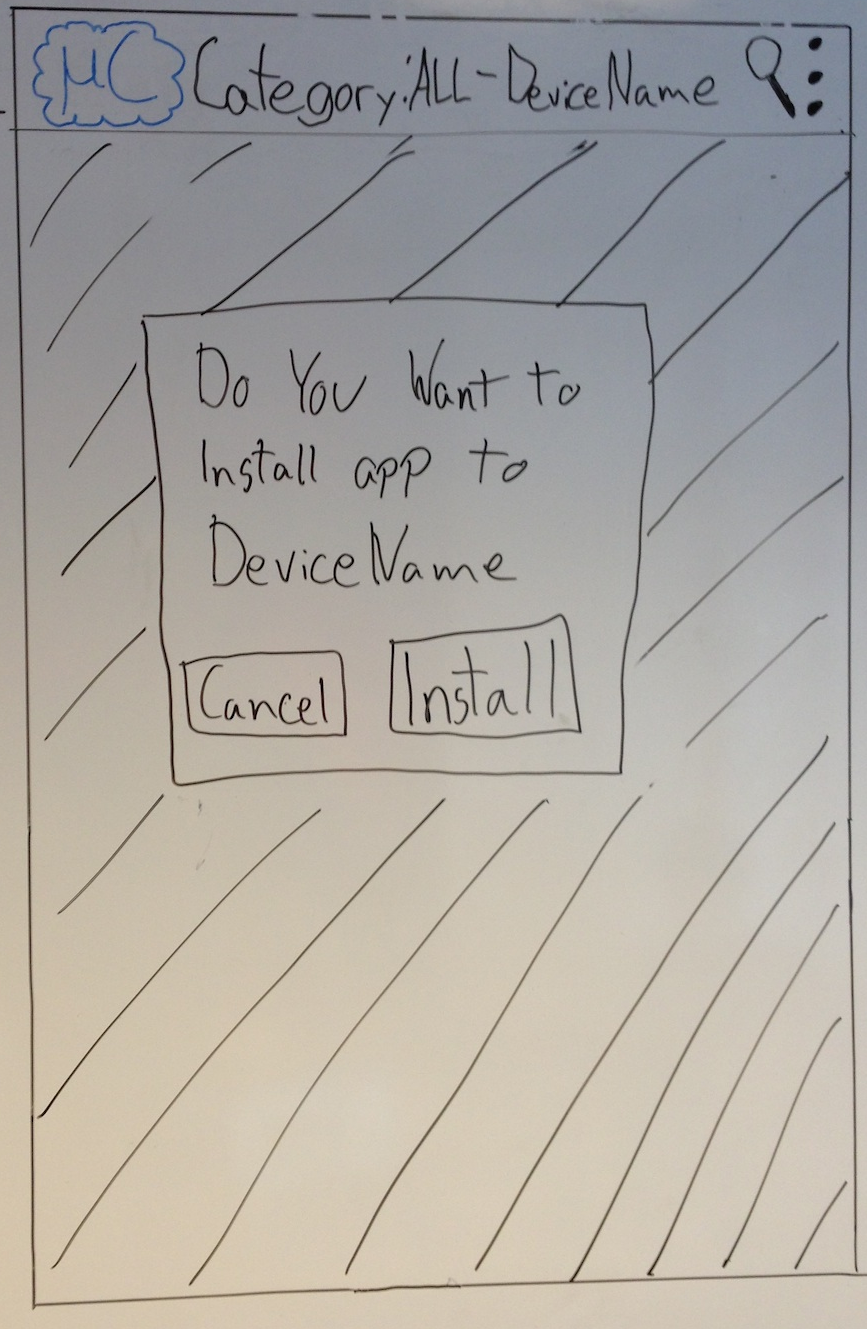
\includegraphics[scale=0.2]{images/Design_guide/Screen3a-i.png}
\caption[Screen 3a-i - Installation confirmation]{When the user click ``install'' , this box will show up to warn and confirm the users choice}
\label{fig:screen3ai}
\end{figure}


\paragraph{Screen 3a-ii - Progress of installation,} as shown in Figure \ref{fig:screen3aii}, is a screen that shows the progress of the installation. The progress bar cannot be dismissed, so the Android application is locked until the installation is complete or has failed.
The user is warned not to move the Android device out of range of the Arduino.

\begin{figure}[H]
\centering
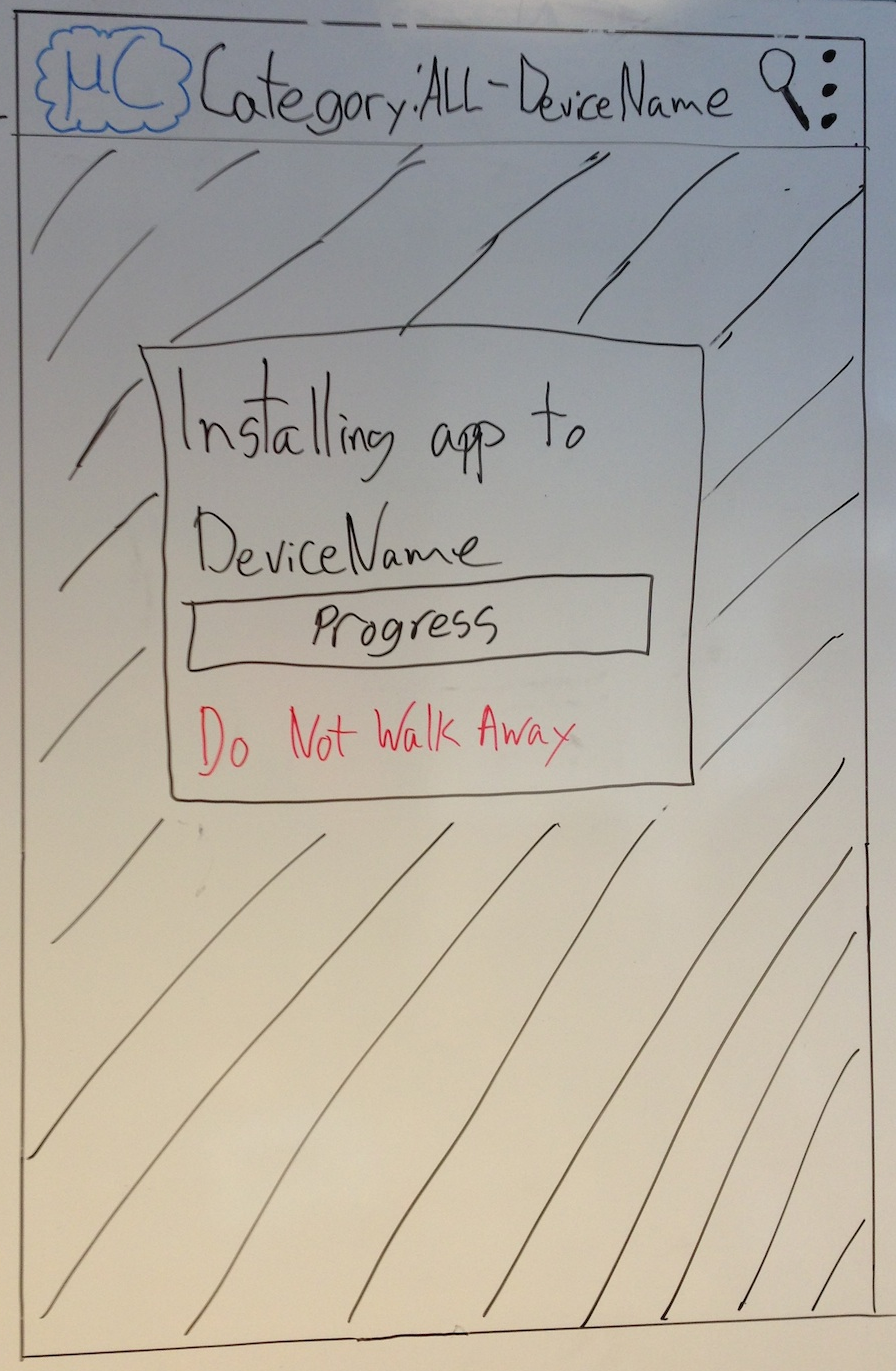
\includegraphics[scale=0.2]{images/Design_guide/Screen3a-ii.png}
\caption[Screen 3a-ii - Progress of installation]{The progressbar that will shop up during the installation over-the-air.}
\label{fig:screen3aii}
\end{figure}


\paragraph{Screen Xa - Action overflow,} as shown in Figure \ref{fig:screenXa}, is a screen that appears when the ``Action overflow'' button is clicked. This menu is available from all the screen in the application with the exception of the preferences screen.

\begin{figure}[H]
\centering
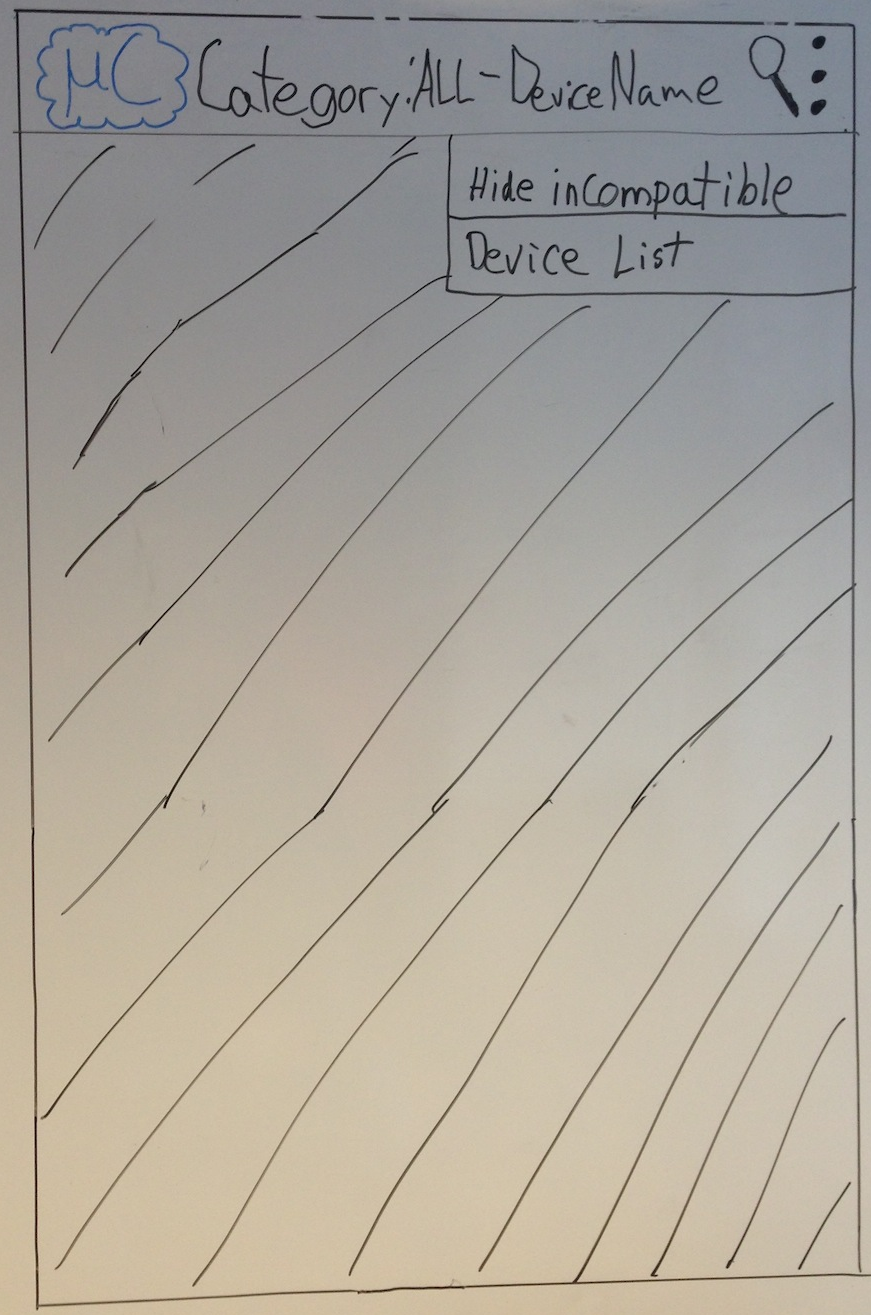
\includegraphics[scale=0.2]{images/Design_guide/ScreenXa.png}
\caption[Screen Xa - Action overflow]{The menu bar that contains settings and properties.}
\label{fig:screenXa}
\end{figure}

	\subsection{Design decisions}
	This section explains the reasoning behind the different aspects of the design.

	\paragraph{Device list.}
	It should be simple and fit as many devices as possible, even on the smaller cell phones. As shown in Figure~\ref{fig:screen1a} it was decided to use discovered Bluetooth devices as a primary method of connecting to an Arduino. The less frequently used methods for connecting to an Arduino, like QR codes and serial input, were put in another screen, as shown in Figure~\ref{fig:screen1b}. \\

	Because of license compatibility issues, it was necessary to use external QR Code readers. To give the user more flexibility, it is therefore possible for the user to select the optimal QR-reader from his application list.\\

	When \textit{Serial input} is clicked, it was decided to open a dialog box for the input string as shown in Figure~\ref{fig:screen1bi}. This is because it clearly gives the user feedback on what is happening and it does not add unnecessary clutter to the GUI.

	\paragraph{Browse shop.}
	The category selection, as shown in Figure~\ref{fig:screen2a} groups the apps in different categories, making it easier for the user to browse for apps. \\

	When a category is chosen, a new screen containing the apps in that category is created. In this screen is it possible for the user to swipe left and right to change the way the apps is sorted. This swiping was implemented because it easily and quickly selects what to show. ``Top hits'' and ``All'' were chosen because the database is currently small, and it is not necessary with a large amount of ``sort by'' tabs. Other tabs could be easily implemented if need be.

	\paragraph{Application view.}
	The application view, as shown in Figure~\ref{fig:screen3a}, should show all the details and information about an application that is useful and interesting to the user. Rating, description, developer and application name were selected for trying to keep a ``standard''. Meaning that both Google Market and AppStore uses these elements and are expected to be familiar to most Android users.\\

	When the ``Install'' button is clicked, a confirmation box will pop up as shown in Figure~\ref{fig:screen3ai}. This is because the user might have clicked the button by accident, or is not informed about what device he or she is connected to. The device name will therefore be shown in this dialog box.\\

	A progress bar will pop up when the user have confirmed the installation. This is because the application should give an indicator on when the application is complete and when its safe to close the application.

	\paragraph{Action overflow menu.}
	When the user clicks on the action overflow menu, he will expect some sort of settings. That is why this menu contains settings. If the user will hide or show incompatible application to his Arduino, this menu will toggle the preference as shown in Figure~\ref{fig:screenXa}.

	\subsection{Changes to the design}
	\label{designchanges}
	In this section the changes made in the design guide will be presented. The final design of the application can be viewed on an Android device.

	\paragraph{Browse shop.}
	In the ``Browse shop'' screen, shown in Figure \ref{fig:screen2a}, the swiping function was removed due to usability issues. Peer reviews indicated that it would be more user friendly to have this as a separate screen, instead of a fragment as shown in the design guide.
	
	\paragraph{Application view.}
	Due to lack of time, some simplifications were made to this screen. It was decided to remove the images and functionality for adding comments was not implemented. 
	
	\paragraph{Action overflow menu.}
	Several different options were added to the Action overflow menu. It is convenient to show different options in this menu, depending on which screen the user is on, so the content of the menu changes throughout the application.

	\paragraph{Add device manually.}
	The ``Bluetooth'' button in Figure \ref{fig:screen1b} was removed, as it was unnecessary.

	\paragraph{Welcome screen.}
	The ``Welcome Screen'' was added as the start screen. This makes it easier to navigate between ``Devices'' and ``Browse Shop''. It also provides an option (checkbox) that allows the user to choose whether or not they will automatically reconnect the next time the application is started. Figure~\ref{fig:welcomescreen} shows a simple connection between the reconnect option and the welcome screen.

	\begin{figure}[H]
	\centering
	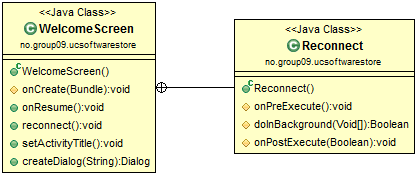
\includegraphics[scale=0.85]{images/UML/welcomescreen.png}
	\caption[UML - Welcome Screen]{The Welcome Screen will reconnect to last connected device if the user have this option enabled. When the user clicks on ``Devices'' or ``Browse Shop'' a new activity is started.}
	\label{fig:welcomescreen}
	\end{figure}

\section{Database implementation}

	SQLite was used as database language because it is integrated with Android and have much functionality that makes it easy to use in an Android application. Because of changes to priorities, the group and the customer agreed to drop the sync adapter, and only use a local database.

	\subsection{Database model}

		In Figure~\ref{fig:erdiagram} the database is shown as an ER Diagram. Established appstore features, like ratings and application pictures, were not important to the customer. Because of this, the \textit{pictures} table was not used.

		\begin{figure}[H]
		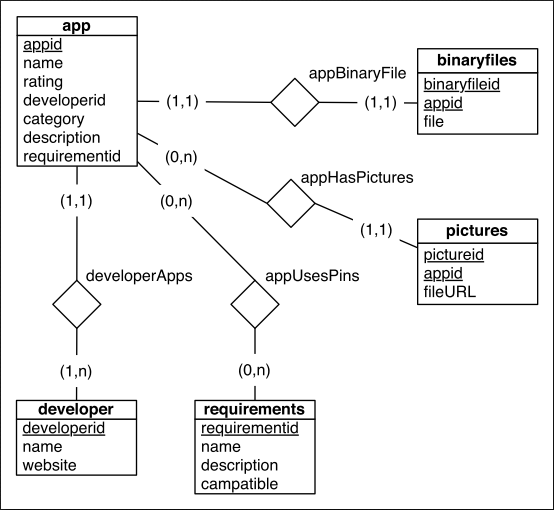
\includegraphics[scale=1]{images/ER_Diagram.png}
		\caption[ER Diagram]{The ER Diagram describing the setup of the database.}
		\label{fig:erdiagram}
		\end{figure}

	\subsection{Database details}

		This section describes the structure and details of the database tables.

		\subsubsection{Table: app}

			This table contains information about the application.\\

			{\bf \underline{appid}(integer):} auto-increment primary key for applications  \\
			\textbf{name(varchar 160):} name of the application \\
			\textbf{rating(int 10):} rating of the application \\
			\textbf{developerid(int 10):} foreign key to the developer of this application \\
			\textbf{category(varchar 200):} which category this application belongs to \\
			\textbf{description(varchar 200):} description of the application \\
			\textbf{requirementid(int 10):} foreign key to the requirements of this application \\

		\subsubsection{Table: binaryfiles}

			This table contains information about the hex-file (compiled Arduino code). \\
			
			{\bf \underline{binaryfileid}(integer):} auto-increment primary key for binary files \\
			\textbf{appid(int 10):} foreign key to the application that owns this binary file \\
			\textbf{file(BLOB 1000000):} The binary file in a BLOB \\

			A BLOB is not a datatype and stores data exactly as it was input. This database stores it as a binary array.

		\subsubsection{Table: developer}

			This table contains information about the developer.\\
			
			{\bf \underline{developerid}(integer):} auto-increment primary key for developers \\
			\textbf{name(varchar 160):} name of the developer \\
			\textbf{website(varchar 200):} website of the developer \\

		\subsubsection{Table: requirements}

			This table contains the requirements for the application.\\
			
			{\bf \underline{requirementid}(integer):} auto-increment primary key for the requirement \\
			\textbf{name(varchar 160):} name of the requirement \\
			\textbf{description(varchar 200):} description of the requirement \\
			\textbf{compatible(int 10):} integer that is converted to boolean when retrieved from database. \\

			Compatible is an integer of 1 or 0. This indicates if the application referred to is compatible with pagers or not.

		\subsubsection{Table: appusespins}

			This table contains the information about which pins on the Arduino that the application is using.\\
			
			\textbf{appid(int 10):} foreign key to the application that uses this rule \\
			\textbf{requirementid(int 10):} foreign key to the associated requirement \\

